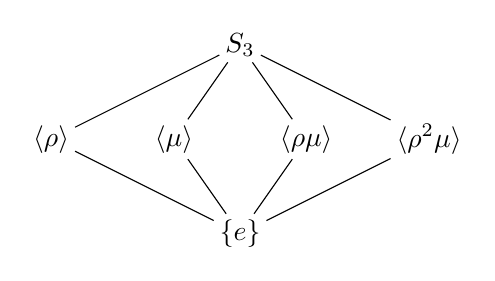
\begin{tikzpicture}[
    every node/.style={inner sep=2pt},
    scale=1.2
  ]
  \node (S3) at (0,2) {$S_3$};
  
  \node (a) at (-2,1) {$\langle \rho \rangle$};
  \node (b) at (-0.7,1) {$\langle \mu \rangle$};
  \node (ab) at (0.7,1) {$\langle \rho\mu \rangle$};
  \node (a2b) at (2,1) {$\langle \rho^2\mu \rangle$};
  
  \node (e) at (0,0) {$\{e\}$};
  
  \draw (S3) -- (a);
  \draw (S3) -- (b);
  \draw (S3) -- (ab);
  \draw (S3) -- (a2b);
  \draw (a) -- (e);
  \draw (b) -- (e);
  \draw (ab) -- (e);
  \draw (a2b) -- (e);
\end{tikzpicture}
